\noindent {\em Auteurs: }\\
De Autopilot gebruikt slechts één algoritme, namelijk om de hoeveelheid thrust te berekenen. De thrust wordt bepaald zodat de drone in rechte lijn naar zijn doel vliegt. Zo vermijdt het onnodig stijgen, dalen en pitch bijstellen. Bovendien kan hierdoor ook de rode bol heel de tijd in beeld blijven. Voor een grafische voorstelling, zie figuur \ref{fig:GrafischeUitwerkingVanHoeveelheidThrustOnderBepaaldePitch}. Hierin is een drone onder een pitch hoek alfa voorgesteld, het zwaartepunt (M) van de rode bol staat relatief ten opzichte van de drone onder hoek beta en zijn ook de krachten drag D, zwaartekracht Fz en thrust T voorgesteld.

\begin{figure}[h]
	\centering
	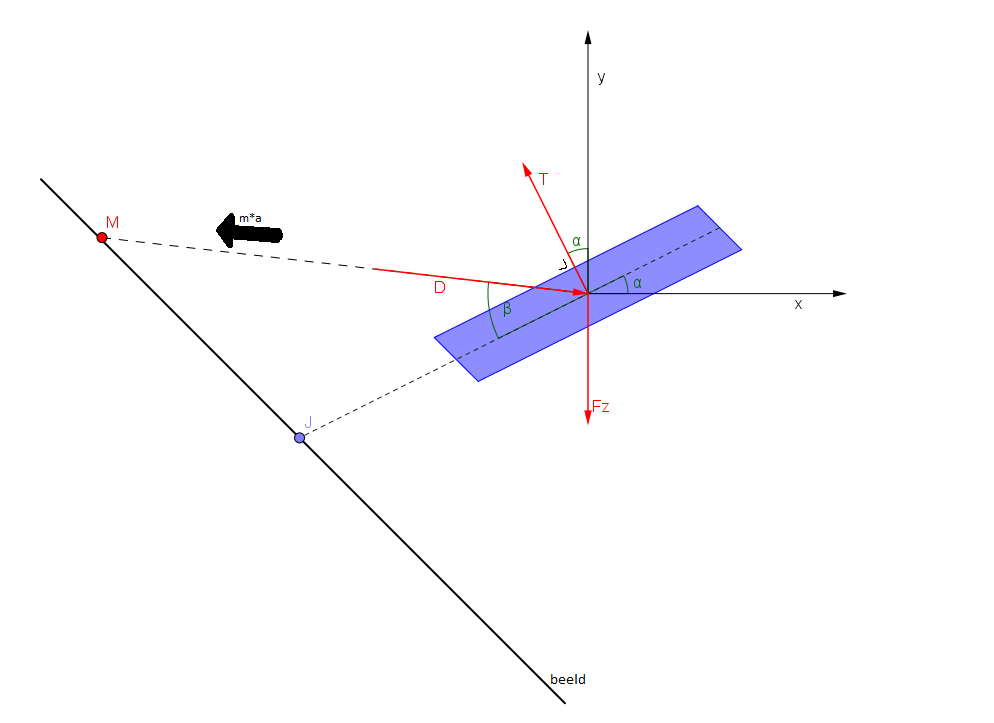
\includegraphics[width=0.8\textwidth]{GrafischeUitwerkingVanHoeveelheidThrustOnderBepaaldePitch.png}
	\caption{Grafische uitwerking van hoeveelheid thrust onder bepaalde pitch hoek.}
	\label{fig:GrafischeUitwerkingVanHoeveelheidThrustOnderBepaaldePitch}
\end{figure}

//TODO dit moet omgezet worden naar echte formules. 
\begin{figure}[h]
	\centering
	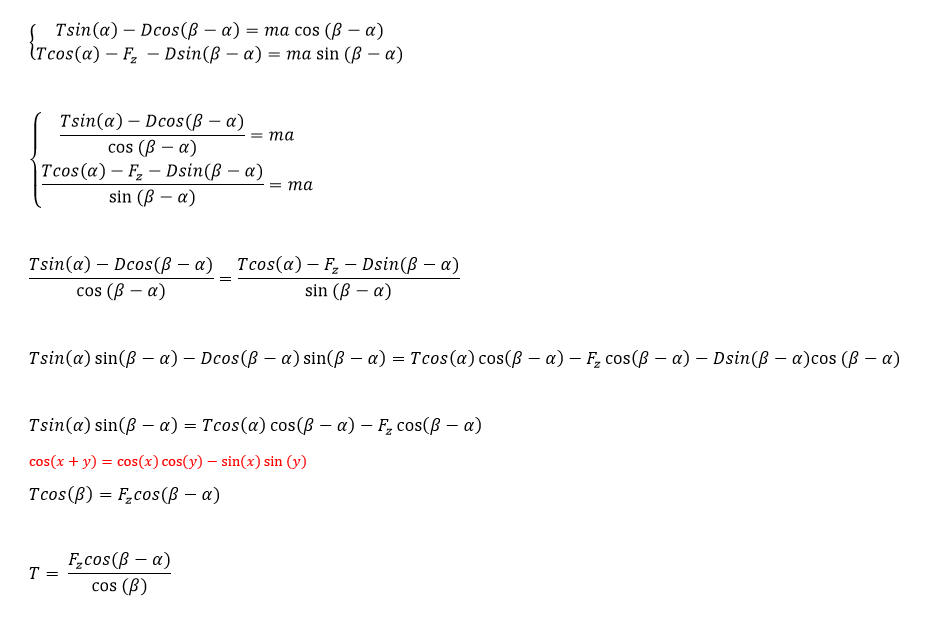
\includegraphics[width=0.8\textwidth]{UitwerkingBerekeningVanHoeveelheidThrustOnderBepaaldePitch.png}
	\caption{Uitwerking van hoeveelheid thrust onder bepaalde pitch hoek.}
	\label{fig:UitwerkingBerekeningVanHoeveelheidThrustOnderBepaaldePitch}
\end{figure}

